\documentclass[11pt]{amsart}
\usepackage[utf8]{inputenc}
\usepackage[T1]{fontenc}
\usepackage{lmodern}
\usepackage{amssymb,amsmath,amsthm}
\usepackage[margin=1.1in]{geometry}
\usepackage{booktabs,array,enumitem}
\usepackage[dvipsnames]{xcolor}
\usepackage{tikz}
\usetikzlibrary{positioning,arrows.meta}
\usepackage[colorlinks=true,linkcolor=blue!50!black,citecolor=green!40!black,urlcolor=blue!50!black]{hyperref}
\renewcommand{\abstractname}{Résumé}
\renewcommand{\refname}{Références}

\newcommand{\Q}{\mathbb{Q}}
\newcommand{\cO}{\mathcal{O}}
\newcommand{\stat}[1]{\textsc{[#1]}}
\newcommand{\Vol}{\mathrm{Vol}}

\title[Synthèse de recherche]{Au-delà du conducteur sans facteur carré dans le théorème réciproque supersingulier en $p=5$ : question, chemin de recherche, résultats et perspectives\\[4pt]\normalfont\small Synthèse de recherche (version française pour lecture)}
\date{Novembre 2026 (brouillon). Détails techniques : note anglaise \emph{« What is new »} (NEW\_RESULTS\_EN.pdf).}

\raggedbottom
\begin{document}
\begin{abstract}
Cette synthèse explique, pour un lecteur spécialiste, la question étudiée, pourquoi elle compte, le chemin suivi (impasses comprises), ce que nous avons obtenu et ce qui pourrait suivre. Chaque énoncé porte l'une des étiquettes suivantes :
\begin{itemize}
\item \stat{prouvé} : argument complet donné ;
\item \stat{confirmé} : confirmé par l'auteur du travail concerné ;
\item \stat{déduction} : esquisse complète, en attente de vérification par un expert ;
\item \stat{ouvert}.
\end{itemize}
Le travail a été mené par un amateur, avec une aide importante d'un système d'IA (Claude). Chaque énoncé cité a été vérifié sur la source.
\end{abstract}
\maketitle

\section{La question}
Bhargava, Skinner et Zhang ont démontré qu'au moins $66{,}48\,\%$ des courbes elliptiques sur $\Q$, rangées par hauteur, vérifient la conjecture de Birch et Swinnerton-Dyer sur le rang [BSZ]. Des théorèmes réciproques $p$-adiques plus récents [BSTW], [Cas] portent ce chiffre à environ $67\,\%$. La méthode combine deux ingrédients :
\begin{itemize}
\item la taille moyenne, égale à $6$, des groupes de $5$-Selmer dans de grandes familles de courbes ;
\item des \emph{théorèmes réciproques $p$-adiques} : un rang de Selmer $r\le1$ entraîne un rang analytique $r$.
\end{itemize}

[BSZ, \S4] remarquent déjà que si leur Théorème~9 pouvait être étendu aux courbes de réduction \emph{supersingulière} en $p$ ([BSZ, Remarque~10]), la borne monterait à $79{,}7\,\%$. [BSTW, Th.~1.6, 12.3] fournissent cette extension pour $p=5$, mais seulement quand le conducteur $N$ est \emph{sans facteur carré}. Or la plupart des courbes de la famille supersingulière $\{5\mid A,\ 5\nmid B\}$ ont une réduction additive en $2$ ou en $3$ : dans la normalisation de [BSZ], environ $92\,\%$ sont supercuspidales en $2$. L'hypothèse « sans facteur carré » fait donc perdre presque tout le gain attendu.

\medskip\noindent\textbf{Question.} \emph{Peut-on retirer l'hypothèse « sans facteur carré » des théorèmes réciproques supersinguliers en $p=5$, au moins aux premiers $2$ et $3$ ? Si oui, jusqu'où monte la borne ?}

Les auteurs eux-mêmes jugent l'hypothèse supprimable : « The hypothesis that $N$ be squarefree is carried over from [CLW22], and it should be removable with some more work » [CLW26, \S1.5(3)].

\section{Où se trouve l'obstacle}
\begin{center}
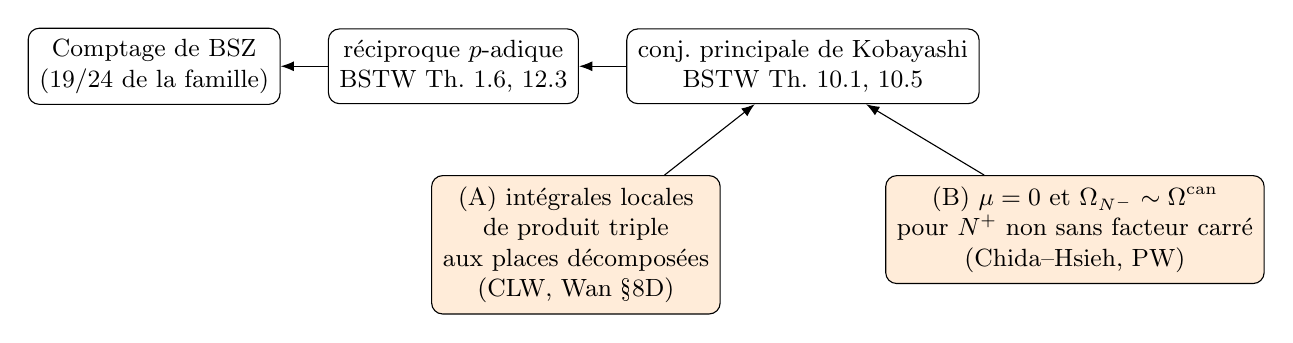
\begin{tikzpicture}[node distance=7mm and 6mm, every node/.style={draw, rounded corners, align=center, font=\small, inner sep=4pt}]
\node (bsz) {Comptage de BSZ\\ ($19/24$ de la famille)};
\node (conv) [right=of bsz] {réciproque $p$-adique\\ BSTW Th.~1.6, 12.3};
\node (k) [right=of conv] {conj.\ principale de Kobayashi\\ BSTW Th.~10.1, 10.5};
\node (A) [below left=9mm and -12mm of k, fill=orange!15] {(A) intégrales locales\\ de produit triple\\ aux places décomposées\\ (CLW, Wan \S8D)};
\node (B) [below right=9mm and -12mm of k, fill=orange!15] {(B) $\mu=0$ et $\Omega_{N^-}\sim\Omega^{\mathrm{can}}$\\ pour $N^+$ non sans facteur carré\\ (Chida--Hsieh, PW)};
\draw[-{Latex}] (conv) -- (bsz);
\draw[-{Latex}] (k) -- (conv);
\draw[-{Latex}] (A) -- (k);
\draw[-{Latex}] (B) -- (k);
\end{tikzpicture}
\end{center}
La lecture de toute la chaîne montre que « $N$ sans facteur carré » n'est utilisé qu'à deux endroits (établi par lecture des sources) :
\begin{enumerate}[label=(\Alph*)]
\item \emph{les intégrales locales de produit triple} : « The square-free-ness was assumed in loc.\ cit.\ for explicit calculation of local triple product periods » [BSTW, note~20] ;
\item \emph{l'invariant $\mu$ et la comparaison des périodes} dans [BSTW, Th.~10.5], qui s'appuient sur [PW] (niveau sans facteur carré).
\end{enumerate}

\section{Chemin de recherche}
\begin{enumerate}[label=\arabic*.]
\item \textbf{(A), première tentative.} Nous avons calculé l'intégrale locale pour $\pi_v$ supercuspidale avec les données locales de [CLW, \S5.6], et trouvé une obstruction. Nous avons ensuite découvert que Fouquet--Wan [FW, Prop.~7.27, Cor.~7.28] traitent exactement ce cas avec un autre choix de données : le vecteur nouveau, et des caractères tels que $\chi_{h,i}\chi_{\theta,i}$ soit non ramifié. Nous avons redémontré leur calcul pour tout $\ell$, y compris $\ell=2$.
\item \textbf{Un test de cohérence qui échoue.} Pour comprendre pourquoi les données de [CLW] diffèrent de celles de [FW], nous avons testé numériquement [Wan, Lemmes 8.13--8.17]. Le Lemme~8.13 se vérifie, mais pas l'énoncé de support du Lemme~8.14.
\item \textbf{Comprendre l'échec.} Un critère de théorie des représentations (la théorie des formes nouvelles de Casselman) montre qu'avec les vecteurs du Lemme~8.17, l'intégrale locale est identiquement nulle. Les fonctions de Schwartz de [CLW, \S7.7] montrent ensuite que les vecteurs de $\theta$ et de $h$ ont la même orientation, comme l'affirme la Remarque~8.19 de Wan. Sur tous ces points, la version publiée de [CLW] est identique.
\item \textbf{Une réparation.} On remplace le vecteur nouveau par le vecteur de fonction de Kirillov $A^{-1}1_{\cO^\times}$, et on ajuste le type des données auxiliaires. On obtient alors une constante non nulle pour \emph{toute} $\pi_v$ générique. La preuve n'utilise que le support de ce vecteur dans le modèle de Kirillov.
\item \textbf{(B).} Nous avons repris [CH, \S5--6] pour $N^+$ quelconque, avec la condition cristalline de [Tay06, \S2] à la place de la condition ordinaire, comme le suggérait déjà [KO, Rem.~6.6]. Cela fait apparaître, en $2$ et $3$, une question de minimalité qui n'existe pas dans le cas sans facteur carré.
\item \textbf{Relecture adverse.} Deux tours d'autocritique hostile : $26$ objections, puis $10$ de plus. Chaque référence a été vérifiée sur la source, et une recherche web a confirmé que rien n'a rendu ce travail caduc.
\item \textbf{Contact avec l'auteur.} X.~Wan a confirmé le cas supercuspidal (voir ci-dessous).
\end{enumerate}


\section{Les Lemmes 8.14 et 8.17 de Wan : ce qu'ils disent, ce que nous avons trouvé}
C'est le cœur de nos résultats sur (A). On se place en un premier décomposé $\ell$, avec $K_t=K_0(\ell^t)$, et $\Phi_f(g)=\langle\pi(g)f,\tilde f\rangle$ le coefficient matriciel d'un vecteur $f$.

\subsection*{Le rôle de ces lemmes}
La preuve de [CLW] (et donc de [BSTW]) a besoin qu'en chaque premier décomposé, un certain nombre, l'\emph{intégrale locale de produit triple} $I_v$, soit \emph{non nul} et indépendant de la famille $p$-adique. [CLW, p.~78] renvoient pour cela à [Wan, Lemmes 8.13--8.17]. Le Lemme~8.17 donne la valeur de $I_v$ :
\[
I_v=\frac{(q-1)^2}{q^{2s+1}}\Vol(K_1)^2\Vol(K_{t_2})^2\neq0,
\]
pour des vecteurs précis ($f_{\chi,\vartheta}$ pour la forme, $f_{\chi_\theta}$ et $f_{\chi_h}$ pour les deux familles auxiliaires). Le Lemme~8.14 est l'étape qui décrit où $\Phi_{f_{\chi,\vartheta}}$ est non nul.

\subsection*{Ce que dit le Lemme 8.14, et pourquoi c'est faux}
\emph{Énoncé} (avec $t<s$) : « si $g\in K_{t+s}$ et $\Phi(g)\neq0$, alors le coefficient en haut à droite de $g$ est divisible par $\varpi^{s-t}$ ».

\emph{Ce que nous trouvons} \stat{prouvé} : pour $g=\begin{pmatrix}1&b\\0&1\end{pmatrix}$, un calcul direct de trois lignes donne
\[
\frac{\Phi(g)}{\Phi(1)}=1\ \text{si } v(b)\ge s-t,\qquad -\frac{1}{q-1}\ \text{si } v(b)=s-t-1,\qquad 0\ \text{sinon}.
\]
Donc $b=\varpi^{s-t-1}$ donne $\Phi(g)\neq0$ alors que $b$ n'est pas divisible par $\varpi^{s-t}$. L'énoncé est faux \emph{pour tous} les $t<s$. Trois calculs numériques indépendants donnent exactement $-1/2$ pour $q=3$. L'énoncé est le même dans la version publiée (ANT 2020).

\subsection*{Ce que dit le Lemme 8.17, et pourquoi la valeur annoncée ne peut pas être la bonne}
\emph{Ce que nous trouvons} \stat{prouvé} : avec ces vecteurs, $I_v=0$ (sauf dans le seul cas $t_1=0$, $s=1$). L'argument tient en quatre lignes et ne dépend pas du Lemme 8.14.
\begin{enumerate}[label=(\roman*)]
\item $f_{\chi_\theta}\otimes f_{\chi_h}$ est un vecteur propre de $K_{t_2}$, de caractère $\Xi$ explicite.
\item L'intégrale d'Ichino est invariante quand on fait agir le même $k$ sur les trois vecteurs ; elle ne voit donc que la projection du premier vecteur sur le type $\Xi^{-1}$.
\item Dans $\pi_f$, ce type n'existe qu'au niveau $c\big(\pi(\chi_{f,1}\chi_{f,2}^{-1}\vartheta,\vartheta)\big)=2s$ (théorie de Casselman), alors que le niveau disponible est $t_2=t_1+s<2s$.
\item La projection est donc nulle, et $I_v=0$, \emph{quel que soit} le vecteur choisi pour la forme.
\end{enumerate}
L'origine probable de l'erreur : le lemme traite $f_{\chi,\vartheta}$ comme s'il était vecteur propre de niveau $t+s$, ce qui est impossible. Le contre-exemple au Lemme 8.14 en est la trace.

\subsection*{Pourquoi cela compte, et ce que nous ne prétendons pas}
\begin{itemize}
\item \emph{Conséquence possible} \stat{déduction}. [CLW] (version publiée, inchangée) utilisent exactement ces lemmes. Si leurs vecteurs locaux sont bien ceux du Lemme 8.17, comme l'écrit Wan (Rem.~8.19), alors la non-nullité annoncée échoue aux premiers décomposés de type série principale ou Steinberg, \emph{même pour $N$ sans facteur carré}. Cela touche une étape de preuve, pas les énoncés finaux.
\item \emph{La correction} \stat{prouvé} : un autre vecteur (fonction de Kirillov $A^{-1}1_{\cO^\times}$, résultat R5) redonne $I_v=\Vol(K_{t_1})\neq0$ pour toute représentation, dans l'esprit de [FW, Prop.~7.27]. Wan a confirmé ce choix dans le cas supercuspidal.
\item \emph{Ce qui reste à confirmer} : que la construction de [CLW] produit bien les vecteurs du Lemme 8.17. C'est la question 1 de la dernière section.
\end{itemize}

\section{Résultats}
\begin{center}\small
\begin{tabular}{p{7.4cm}p{2.3cm}p{4.2cm}}
\toprule
Résultat & Statut & Commentaire\\ \midrule
R1. L'énoncé de support de [Wan, Lemme~8.14] (ANT 2020) est faux pour tout $s>t$ : $\Phi(n(\varpi^{s-t-1}))=-\Phi(1)/(q-1)\neq0$. & \stat{prouvé} & preuve de trois lignes ; trois vérifications numériques indépendantes\\
R2. Avec les vecteurs de [Wan, Lemme~8.17], l'intégrale locale d'Ichino vaut $0$ (sauf $t_1=0$, $s=1$). & \stat{prouvé} & preuve courte via [Cas73, Th.~1] ; indépendant de R1\\
R3. Avec les données locales (4) de [CLW] (version publiée, p.~39 et 78), l'intégrale locale s'annule aux places décomposées où $\pi_v$ est ramifiée, déjà pour $N$ sans facteur carré. & \stat{déduction} & repose sur l'identification des vecteurs locaux affirmée en [Wan, Rem.~8.19]\\
R4. Places décomposées supercuspidales : le choix de [FW, Prop.~7.27] fonctionne. & \stat{confirmé} & X.~Wan, communication privée (citation sous réserve de son accord)\\
R5. Pour toute $\pi_v$ générique, le vecteur $\phi_A$, avec des données assorties, donne $I_v=\Vol(K_{t_1})\neq0$, indépendant de la famille. & \stat{prouvé} modulo [Wan, Lemme~8.13] & vérifications numériques en $\ell=2,3$\\
R6. (B) pour $N^+$ quelconque au niveau minimal : version cristalline de [CH, Prop.~6.8]. & \stat{déduction} & étapes suivies dans [Tay06, \S2]\\
R7. Les configurations non minimales (E1)--(E3) en $2$ et $3$ sont réelles (définition standard [KO, Déf.~3.5]). & \stat{prouvé} & exclues du chiffrage\\
R8. La tordue $g_K$ aux premiers divisant $D_K$ (rang $1$) est laissée ouverte aussi dans [BSTW]. & \stat{ouvert} & point hérité\\ \bottomrule
\end{tabular}
\end{center}

\section{Ce que cela pourrait donner}
\begin{center}\small
\begin{tabular}{p{8.3cm}l}
\toprule
Scénario & proportion\\ \midrule
Aujourd'hui (BSZ + BSTW + Castella) & $67{,}02\,\%$\\
(A) pour tous les types via R4/R5, (B) via R6, sans (E1)--(E3) ; conditionnel à R8 et à une validation par des experts & $\mathbf{78{,}61\,\%}$\\
Idem, en récupérant (E1)--(E3) (via [Dia97b] et un argument de torsion) & $79{,}03\,\%$\\
En utilisant aussi $p=3$ (suggéré dans [BSZ, \S4]) & $>80\,\%$ (non calculé)\\ \bottomrule
\end{tabular}
\end{center}
\noindent Il y a aussi deux sous-produits, indépendants de la borne :
\begin{itemize}
\item R1--R3 portent sur un calcul local publié, utilisé par [CLW], et à travers lui par [BSTW] et [CLW26] ;
\item R5 fournit un remplacement uniforme de ce calcul.
\end{itemize}

\section{Ce que nous aimerions savoir}
\begin{enumerate}
\item R2 et R3 sont-ils corrects, c'est-à-dire les vecteurs du Lemme~8.17 sont-ils bien ceux utilisés aux places décomposées ? R5 rétablit-il l'argument aux places de série principale et de Steinberg ?
\item La condition (4) de [CLW] au premier auxiliaire $\ell$ est-elle compatible avec la torsion par $\nu$ ?
\item Dans (B), le Lemme~6.5 de [CH] est-il correct dans les configurations (E2) et (E3) ? Comment traiter la tordue $g_K$ aux premiers $\ell\mid D_K$ (R8) ?
\end{enumerate}
Tout ceci est indépendant de toute hypothèse de Riemann : les arguments sont locaux et $p$-adiques.

\section*{Petit lexique (pour la lecture)}
\begin{description}[font=\normalfont\itshape, leftmargin=0pt]
\item[Lemme] petit résultat intermédiaire servant à démontrer un résultat principal.
\item[Intégrale locale de produit triple] un nombre calculé en chaque premier, qui doit être non nul (et indépendant de la famille) pour que la preuve globale de CLW fonctionne.
\item[Place décomposée] un premier qui se scinde en deux dans le corps quadratique auxiliaire ; $2$ et $3$ sont choisis ainsi.
\item[Supercuspidale, série principale, Steinberg] les trois grands types de comportement local d'une courbe en un premier où elle a mauvaise réduction.
\item[Invariant $\mu$, périodes] le problème B : contrôler la divisibilité par $p$ d'une fonction $L$ $p$-adique, et comparer deux normalisations.
\item[Minimal] au niveau minimal, aucune forme modulaire « parasite » d'un autre type n'est congruente à la nôtre au même niveau.
\end{description}

\begin{thebibliography}{BSTW}\small
\bibitem[BSZ]{BSZ} M.~Bhargava, C.~Skinner, W.~Zhang, \emph{A majority of elliptic curves over $\Q$ satisfy the BSD conjecture}, arXiv:1407.1826.
\bibitem[BSTW]{BSTW} A.~Burungale, C.~Skinner, Y.~Tian, X.~Wan, \emph{Zeta elements for elliptic curves and applications}, arXiv:2409.01350.
\bibitem[Cas]{Cas} F.~Castella, \emph{Exceptional zeros for Heegner points and $p$-converse\dots}, arXiv:2409.01360.
\bibitem[Cas73]{Cas73} W.~Casselman, \emph{On some results of Atkin and Lehner}, Math.\ Ann.\ 201 (1973).
\bibitem[CH]{CH} M.~Chida, M.-L.~Hsieh, \emph{Special values of anticyclotomic $L$-functions for modular forms}, J.\ reine angew.\ Math.\ 741 (2018).
\bibitem[CLW]{CLW} F.~Castella, Z.~Liu, X.~Wan, Forum Math.\ Sigma 10 (2022), e110.
\bibitem[CLW26]{CLW26} F.~Castella, Z.~Liu, X.~Wan, \emph{Kato's main conjecture for nonordinary modular forms}, arXiv:2608.29470.
\bibitem[Dia97b]{Dia97b} F.~Diamond, Invent.\ Math.\ 128 (1997).
\bibitem[FW]{FW} O.~Fouquet, X.~Wan, arXiv:2107.13726.
\bibitem[KO]{KO} C.-H.~Kim, K.~Ota, arXiv:1905.02926.
\bibitem[PW]{PW} R.~Pollack, T.~Weston, Compos.\ Math.\ 147 (2011).
\bibitem[Tay06]{Tay06} R.~Taylor, Doc.\ Math.\ (2006).
\bibitem[Wan]{Wan} X.~Wan, Algebra Number Theory 14 (2020), 383--483.
\end{thebibliography}
\end{document}
